\subsection{Problem}
\renewcommand{\theequation}{\theenumi}
\begin{enumerate}[label=\thesection.\arabic*.,ref=\thesection.\theenumi]
\numberwithin{equation}{enumi}

\item The points scored by a Kabaddi team in a series of matches are as follows: 17, 2, 7, 27, 15, 5, 14, 8, 10, 24, 48, 10, 8, 7, 18, 28 .Find the median of the points scored by the team.

\solution  Arranging the points scored by the  team in ascending order we get:\\
2,5,7,7,8,8,10,10,14,15,17,18,24,27,28,48\\
Let N be the no. of observations = 16\\
\begin{align}
\text{Median} = \frac{\brak{\frac{N}{2}}^{th}\text{value} + \brak{\frac{N}{2}+1}^{th}\text{value}}{2}
\end{align}

\begin{align}
\text{Median} &= \frac{\brak{8}^{th}\text{value} + \brak{9}^{th}\text{value}}{2}\\
\text{Median} &= \frac{10 + 14}{2}\\
\text{Median} &= 12
\end{align}
\begin{comment}
	\begin{lstlisting}
	./codes/triangle/q2.py
	\end{lstlisting}
	
	\begin{figure}[!ht]
	\centering
	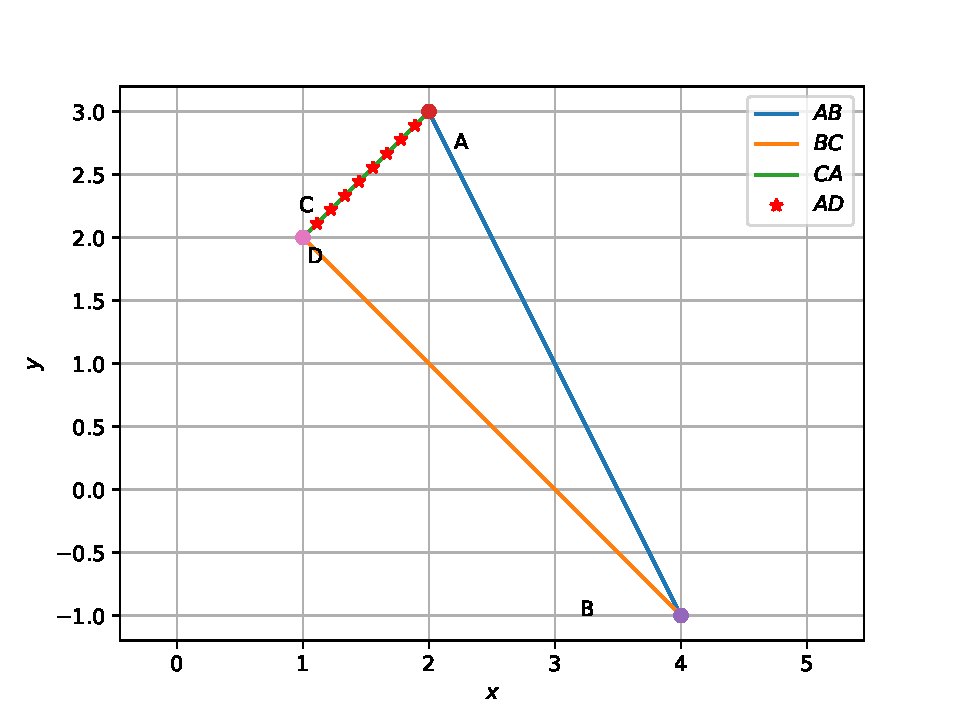
\includegraphics[width=\columnwidth]{./figs/triangle/q2.pdf}
	\caption{Triangle of Q.1.2.5}
	\label{fig:qtwo}	
	\end{figure}
	

\end{comment}	
	
	
\end{enumerate}
